\def\year{2020}\relax

\documentclass[letterpaper]{article} %DO NOT CHANGE THIS
\usepackage{aaai20}  %Required
\usepackage{times}  %Required
\usepackage{helvet}  %Required
\usepackage{courier}  %Required
\usepackage{url}  %Required
\usepackage{graphicx}  %Required
\frenchspacing  %Required
\setlength{\pdfpagewidth}{8.5in}  %Required
\setlength{\pdfpageheight}{11in}  %Required
\setcounter{secnumdepth}{0}  
\usepackage{subfigure}
\usepackage{xcolor}
\usepackage[linesnumbered,ruled]{algorithm2e}
\usepackage{amsmath}
\usepackage{dblfloatfix}    % To enable figures at the bottom of page

\makeatletter
\newcommand{\removelatexerror}{\let\@latex@error\@gobble}
\makeatother
\begin{document}
% The file aaai.sty is the style file for AAAI Press 
% proceedings, working notes, and technical reports.
%
\title{A Genetic Approach to the Formulation of Tetris Engine}
\author{Jiachen Zhang, Miaoqi Zhang, Shuheng Cao\\
\{j756zhan, m337zhan, s53cao\}@uwaterloo.ca\\
University of Waterloo\\
Waterloo, ON, Canada\\
}
\maketitle
\newcommand\bi[1]{{\textcolor{blue}{#1}}}
%%%%%%%%%. Abstract %%%%%%%%%

\begin{abstract}
{\bf Complete this section for D4.}

The {\it Abstract} should be at most 150 words long, and should summarize briefly what your project is about.  This includes the motivation for the problem (2-3 sentences), the problem you tackled (2-3 sentences), and your main results (1-2 sentences).   
\end{abstract}

%%%%%%%%%. Introduction %%%%%%%%%

\section{Introduction} 

% The {\it Introduction} section ($\sim$1 page) describes the background and motivation behind your work, and provides an overview of the work and the findings.  It should include the following content.  
%
\begin{itemize} 

\item 
{\bf Motivations}
% {\bf Complete this part for D1.}

% Motivate your entire paper.  At a high level, describe the problem that your project is addressing.  Why is this an important problem to tackle?  If there a solution to this problem, what are some potential real-world impacts of this solution?  Try to give a compelling motivating story.  If possible, support your argument with evidence such as facts and statistics.  (2-3 paragraphs)

With the great triumph of AlphaGo in 2016, more and more researchers are interested in using machine learning techniques to solve more advanced and complicated games such as StarCraft II. However, in the authors' opinion, it also provides us an invaluable opportunity to revisit some of the traditional video games, aiming for more reliable and satisfying results. Consequently, this project's primary motivation is to introduce, implement, and compare several different approaches to tackle the Tetris, a tile-matching video game with enduring appeal and popularity. A more detailed introduction and instruction of Tetris will be presented in the {\it Methodology} section since the authors implemented a Tetris in Python for visualization and illustration purpose.

Solving Tetris is a crucial and intriguing topic due to the two reasons below. On the one hand, Tetris is essentially an extraordinary optimization problem because each game will end no matter how well they are placed \cite{burgiel_1997}, so there is no such thing as perfect solutions to Tetris and there is always room to improve. On the other hand, the analyses and comparisons mentioned in this report are not limited to Tetris only, where we could broaden them to real-life problems, such as self-driving cars and robotics, {with appropriate modifications on the architectures introduced in this article}.

Finally, as mentioned in the {\it Discussion} section, one of the main problems the machine learning community faces is the lack of explainability and interpretability for most of the models. The direct analyses on most of the recent models, such as AlphaGo and AlphaZero, are notoriously complicated and challenging, but with a more straightforward and simplified setup like Tetris, it gives us more opportunities to have a more in-depth insight into what is happening under the hood. Consequently, the results from simple setups will contribute to a better and deeper understanding of the more complex models.

\item 
{\bf Methodologies}
% {\bf For D1, describe the problem and your methodologies only.  Then, complete this part for D4. }

% Describe, at a high-level, the problem you tackled and your main results.  What research questions are you trying to answer?   What methodologies did you used to answer the question? What are the performance measures that you used to evaluate the methodologies?   Describe your key findings in 2-3 sentences. (2-3 paragraphs)
In brief, the methodology of this project consists of four main parts, as shown below.
\begin{itemize}
  \item 
  First and foremost, we built a Tetris interface for both visualization and training purposes. For the sake of communication with our models, the interface is written in Python. 
  \item 
  Next, we {will solve} the problem using a hand-crafted agent. {Inspired by Bertsekas and Tsitsiklis's paper} \cite{Bertsekas_1996}, we will manually chose the weights for 4 most representative state features: the number of holes, the height of the highest column, the height of each column, and the difference in height between consecutive columns. This approach is based mainly on the heuristic search algorithm and involves a lot of trails-and-errors. The result serves as the benchmark for the project {using the evaluation metrics mentioned below}.
  \item 
  On top of that, we will also tackle the problem {using local search algorithm}. The main idea is to use a genetic algorithm to automatically find an optimal weight combination for 9 state features, where the detailed description for the features could be found in the Methodology section. 
  % {According to the nature of the local search algorithm, this method will find the optimal weights without any human interference, and consequently, it is able to rely on more state features compared with the hand-crafted agent. As a result, we expect the local search algorithm to outperform the benchmark.}
  
  % After 200 training epochs, we indeed get a result surpassed the benchmark.
  \item {Ultimately, we will solve the problem with reinforcement learning. The main idea is that we will build and train a deep Q-network (DQN) to evaluate all the successor states of the current state. More precisely, the DQN will receive a bitmap representation of successor and output a non-negative number represents the score for it. The agent will choose the successor with the highest score with probability $\epsilon$ and otherwise, it will select a random successor.}
  % Ultimately, we added more functionalities to the traditional Tetris, like introduce the ability to see the next Tetromino and enable holding the unwanted Tetromino, and the retrained model yields satisfying results, which proved the ability to generalization.

\end{itemize}
{As for the evaluation metric, we will use the number of lines cleaned up before game over as our primary metric so that we could compare the three methods with each other as well as implementations from other papers. One thing worth mention is that in the DQN training, we won't directly use the evaluation metric mentioned above as the reward because it is too sparse. Instead, we will design a reward that is positively correlated with the evaluation metrics. More concretely, we will use the following rewarding scheme:}
\begin{table}[h!]
  \centering
  \normalsize{
    \begin{tabular}{ |c|c| } 
      \hline
      Situation & Reward  \\ 
      \hline
       Game over & $-100$  \\ 
       \hline
       Clean up $k$ lines & $10\times k^{2}$  \\ 
       \hline
       Safely landing a piece & $1$  \\
       \hline
       Otherwise & $0$  \\
       \hline
      \end{tabular}}
  \caption{Reward Function}
  \label{tab:reward}
\end{table} 

\item 
{\bf Complete this bullet point for D4.}

Emphasize your contributions.  How should we interpret the results?  Why should people care about this work?   Does this project introduce any novel techniques or reveal any unexpected findings?  In bullet point forms, list 3-4 key contributions of your project.

\end{itemize}

%%%%%%%%%. Related Work %%%%%%%%%

\section{Related Work} 

There is a number of algorithms about Tetris so far. Most algorithms for Tetris use features and a linear evaluation function \cite{SO19}. The algorithms define multiple features and assign a weight value to each of the features. For a specific state with an existing Tetromino, it will use the evaluation function to calculate the evaluation value according to the weight of the features for every possible states. And then a "best" placement of the Tetromino will be picked according to the evaluation value.

Tracing back to 1996, J.N. Tsitsiklis and B. Van Roy formulated Tetris as a Markov Decision problem. They introduced Feature-Based Method for Large Scale Dynamic Programming. The algorithm introduced two features, which were the number of "holes" and the height of the tallest column. Each state will be represented as a two-hundred-dimensional binary vector since the Tetris board is form by $10 \times 20$ grids. And a seven-dimentional bianry vector will represent the current falling Tetromino since there are seven type of Tetrominos in total. The algorithm can eliminate 31 rows on average of a hundred games \cite{TV96}.

Later on, more features have been taken into consideration. For example, peak height, landing height, number of holes, row transition, column transition and eroded piece cells \cite{WCWT}. 

These features were identified by the best artificial Tetris player until 2008 and introduced evalutation function: 
$-4 \times holes - cumulative\ cells - row\ transitions - column\ transitions - landing\ height + eroeded\ cells$ \cite{SO19}. However, most algorithm will perform a row elimination whenever it is possible. This is not optimal in the long term because there could be some state that multiple rows can be eliminated at once \cite{WCWT}. 

Tsai, Yen, Ma and Yu implemented "Tetris A.I.". Scores will be rewarded if a I-Tetromino is dropped and 4 rows are eliminated. The main idea is to make this kind of move as many as possible. The solution for this is to stack on the 9 columns and remain the left column empty. As long as an I-Tetromino apprears, it will be drop at that seperate column to eliminate multiple rows \cite{WCWT}.

Moreover, they also implemented another model called "Two Wide Combo A.I.", which is a little bit more complex than the previous algorithms. It breaks the process into two parts. One is to "Stack" on the left eight columns by using BFS, and the other part is "Combo", which is to eliminate rows consecutively to earn Combo Bonus by dropping Tetrominos into the rest two columns \cite{WCWT}.

The use of generic algorithm provides a new way which is worth taking into consideration. In 2006, Szita and Lorincz implemented cross-entropy algorithm. New features were introduced and for each feature, multiple games were played. It took the mean and standard deviation of the best weight of the linear policy that maximize the score and generated a new generation of policies \cite{SO19}.

Back in 2003, Thomas Gärtner, Kurt Driessens and Jan Ramon introduced a new approach to Tetris optimization\cite{s017}. What's innovative in this paper is that researchers primarily used Relational Reinforcement Learning (RRL), training the network with Gaussian processes and graph kernels. Relational Reinforcement Learning advances traditional Reinforcement Learning by integrating with a relational learning programming which is also known as inductive logic programming. The use of Gaussian processes is to make probabilistic predictions and allow the agent to incrementally perform learning tasks. On the other hand, graph kernels help represent various states and actions during training process in a more structural way, which greatly facilitates learning. Compared to some previous RRL models which train data based on techniques such as decision trees, this approach has proven to be more effective.

In 2016, researcher at Stanford University continued to optimize Tetris engine performance using Reinforcement Learning \cite{s016}. They used a notation called Q function. This function evaluate actions taken by the AI at various stages/states during the game; the value of this Q function tells us what the best next action is. Researchers attempted to improve convergence of Q function with the aid of heuristic functions. This method yields the best performance when combined with grouping actions. Basically, grouping actions means the entire sequence of actions a single piece take as it drops to the bottom whereas a single action is just one movement of the piece such as one space to the left. Although grouped actions increase game length compared to single actions, they achieved a much high game score. Another technique that significantly boosts the performance is transfer learning. Transfer learning effectively scores an average of two lines per game, compared to no lines for learning from scratch. The final technique used is called prioritized sweeping. Prioritized sweeping involves calculating a priority value. Based on that value, the researchers sampled actions based on probabilities proportionally to their priorities. This technique solves several problems, for example, the issue that certain actions gotten drastically under-represented in the experience dataset.

%%%%%%%%%. Methodology %%%%%%%%%

\section{Methodology}

\subsection{Handcrafted Agent}
\subsection{Local Search Agent}
\subsection{Reinforcement Learning Agent}

The genetic algorithm mentioned above is intelligent in the sense that it will automatically find optimal weight combinations. However, notice that it is still not perfect because the state features are always chosen by humans, and they are not necessarily representative. More concretely, we may lose some information since we will represent all the successors' states, which is of size $20\times 10$, using only nine features. Thus, we will develop a new algorithm that eliminates human-chosen features and finds a feasible representation itself.

As a result, we naturally lean towards the fields of reinforcement learning and will start with the Q-learning introduced by Chris Watkins in 1989. The detailed deduction and convergence proof are pretty complicated and are out of the scope of this report. However, the final results of Q-learning are incredibly similar to dynamic programming, where we maintain a Q-table with current states $s_i$ as column and available actions $a_j$ as rows:

\begin{table}[h!]
  \centering
  \normalsize{
    \begin{tabular}{ |c|c|c|c|c|c| } 
      \hline
       & $a_{0}$ & $a_{1}$ & $\cdots$ & $a_{n}$  \\ 
      \hline
       $s_{0}$ & $0.91$ & $0.65$ &$\cdots $ &$0.45$  \\ 
       \hline
       $s_{1}$ & $0.86$ & $0.14$ &$\cdots $ &$0.19$  \\ 
       \hline
       $\vdots$ & $\vdots$ & $\vdots$ &$\ddots $ &$\vdots$  \\ 
       \hline
       $s_{m}$ & $0.26$ & $0.61$ &$\cdots $ &$0.27$  \\ 
       \hline
      \end{tabular}}
  \caption{Q-table example with random initialization}
  \label{tab:qtable}
\end{table}
% Table \ref{tab:reward}
% \begin{align*}
  % \end{align*}
And for each step, we will update the entry $(s_{t}, a_{t})$ using the formula
\[
    % Q^{new}(s_{t},a_{t}) \leftarrow \underbrace{Q(s_{t},a_{t})}_{\textit{old value}} + \underbrace{\alpha}_{\textit{learning rate}} \cdot  \overbrace{\bigg( \underbrace{\underbrace{r_{t}}_{\textit{reward}} + \underbrace{\gamma}_{\textit{discount factor}} \cdot \underbrace{\max_{a}Q(s_{t+1}, a)}_{\textit{estimate of optimal future value}}}_{\textit{new value (temporal difference target)}} - \underbrace{Q(s_{t},a_{t})}_{\textit{old value}} \bigg) }^{\textit{temporal difference}}
    Q(s_{t},a_{t}) \leftarrow (1-\alpha) Q(s_{t},a_{t}) + \alpha   \left ( r_{t} + \gamma  \max_{a}Q(s_{t+1}, a)\right ) 
\]
where we have two hyper-parameters embedded in this formula:
\begin{itemize}
  \item $\alpha$: learning rate, which determines to what extent newly acquired information overrides old information.
  \item $\gamma$: discount factor, which determines the importance of future rewards.\footnote{The term $\max_{a}Q(s_{t+1}, a) $ represents the estimation of the optimal future value.}
\end{itemize}

On top of that, we also need to manually determine three important setups:
\begin{itemize}
  \item $s_{i}$: all the possible states for the environment represented by a $20\times 10$ bitmap.
  \item $a_{j}$: all the possible actions a player can take for a state.
  \item $r_{t}$: reward received when moving from the state $s_{t}$ to $s_{t+1}$ and is determined by the reward function.
\end{itemize}

With all these hyper-parameters and setups, we will let the agent interact with the environment on its own. At each state, the agent will always choose to perform the action with the highest Q-value and update the Q-table according to the updating formula.\footnote{Here, it is not always true that the agent will perform the action with the highest Q-value. Some techniques like $\epsilon$-greedy algorithm will choose the optimal action with probability $\epsilon$ and a random walk otherwise. We will talk more about this in the experimental design section.} We will stop Q-learning until the agent completes the game, and we will repeat this process for large enough epochs so that the Q-table converges.

Now, we will begin with a naive adaptation to the Tetris by defining states to be all the possible game states for a Tetris board of size $20\times 10$ and defining actions to be the set $\{clockwise\,\,rotation$, $counter\textit{-}clockwise\,\,rotation$, $left$, $right$, $down\}$.
% $\{\textit{left},\textit{right}, \textit{down},\textit{clockwise rotation}, \textit{counter-clockwise rotation}\}$.

Theoretically, we could tackle this Tetris problem directly using the Q-learning setups mentioned above, but we are facing two severe hindrances:
\begin{enumerate}
  \item The reward is very sparse because all the actions except down are perfectly reversible. For example, $left$ can be reversed by $right$, and $clockwise\,\,rotation$ can be reversed by $counter\textit{-}clockwise\,\,rotation$. As a result, in the exploration stage, it will take the agent a long time before it can achieve a reward, which is particularly bad for training.
  \item Furthermore, according to Phon-Amnuaisuk's paper, the number of stable states for a $20\times 10$ Tetris board is in the order of $10^{60}$ \cite{somnuk_2015}, which means our Q-table will be of size approximately $5\times 10^{60}$. This table is way too large to store in RAM and the training time for such a large table is also unbearable.
\end{enumerate}

\begin{figure}
  \centering
  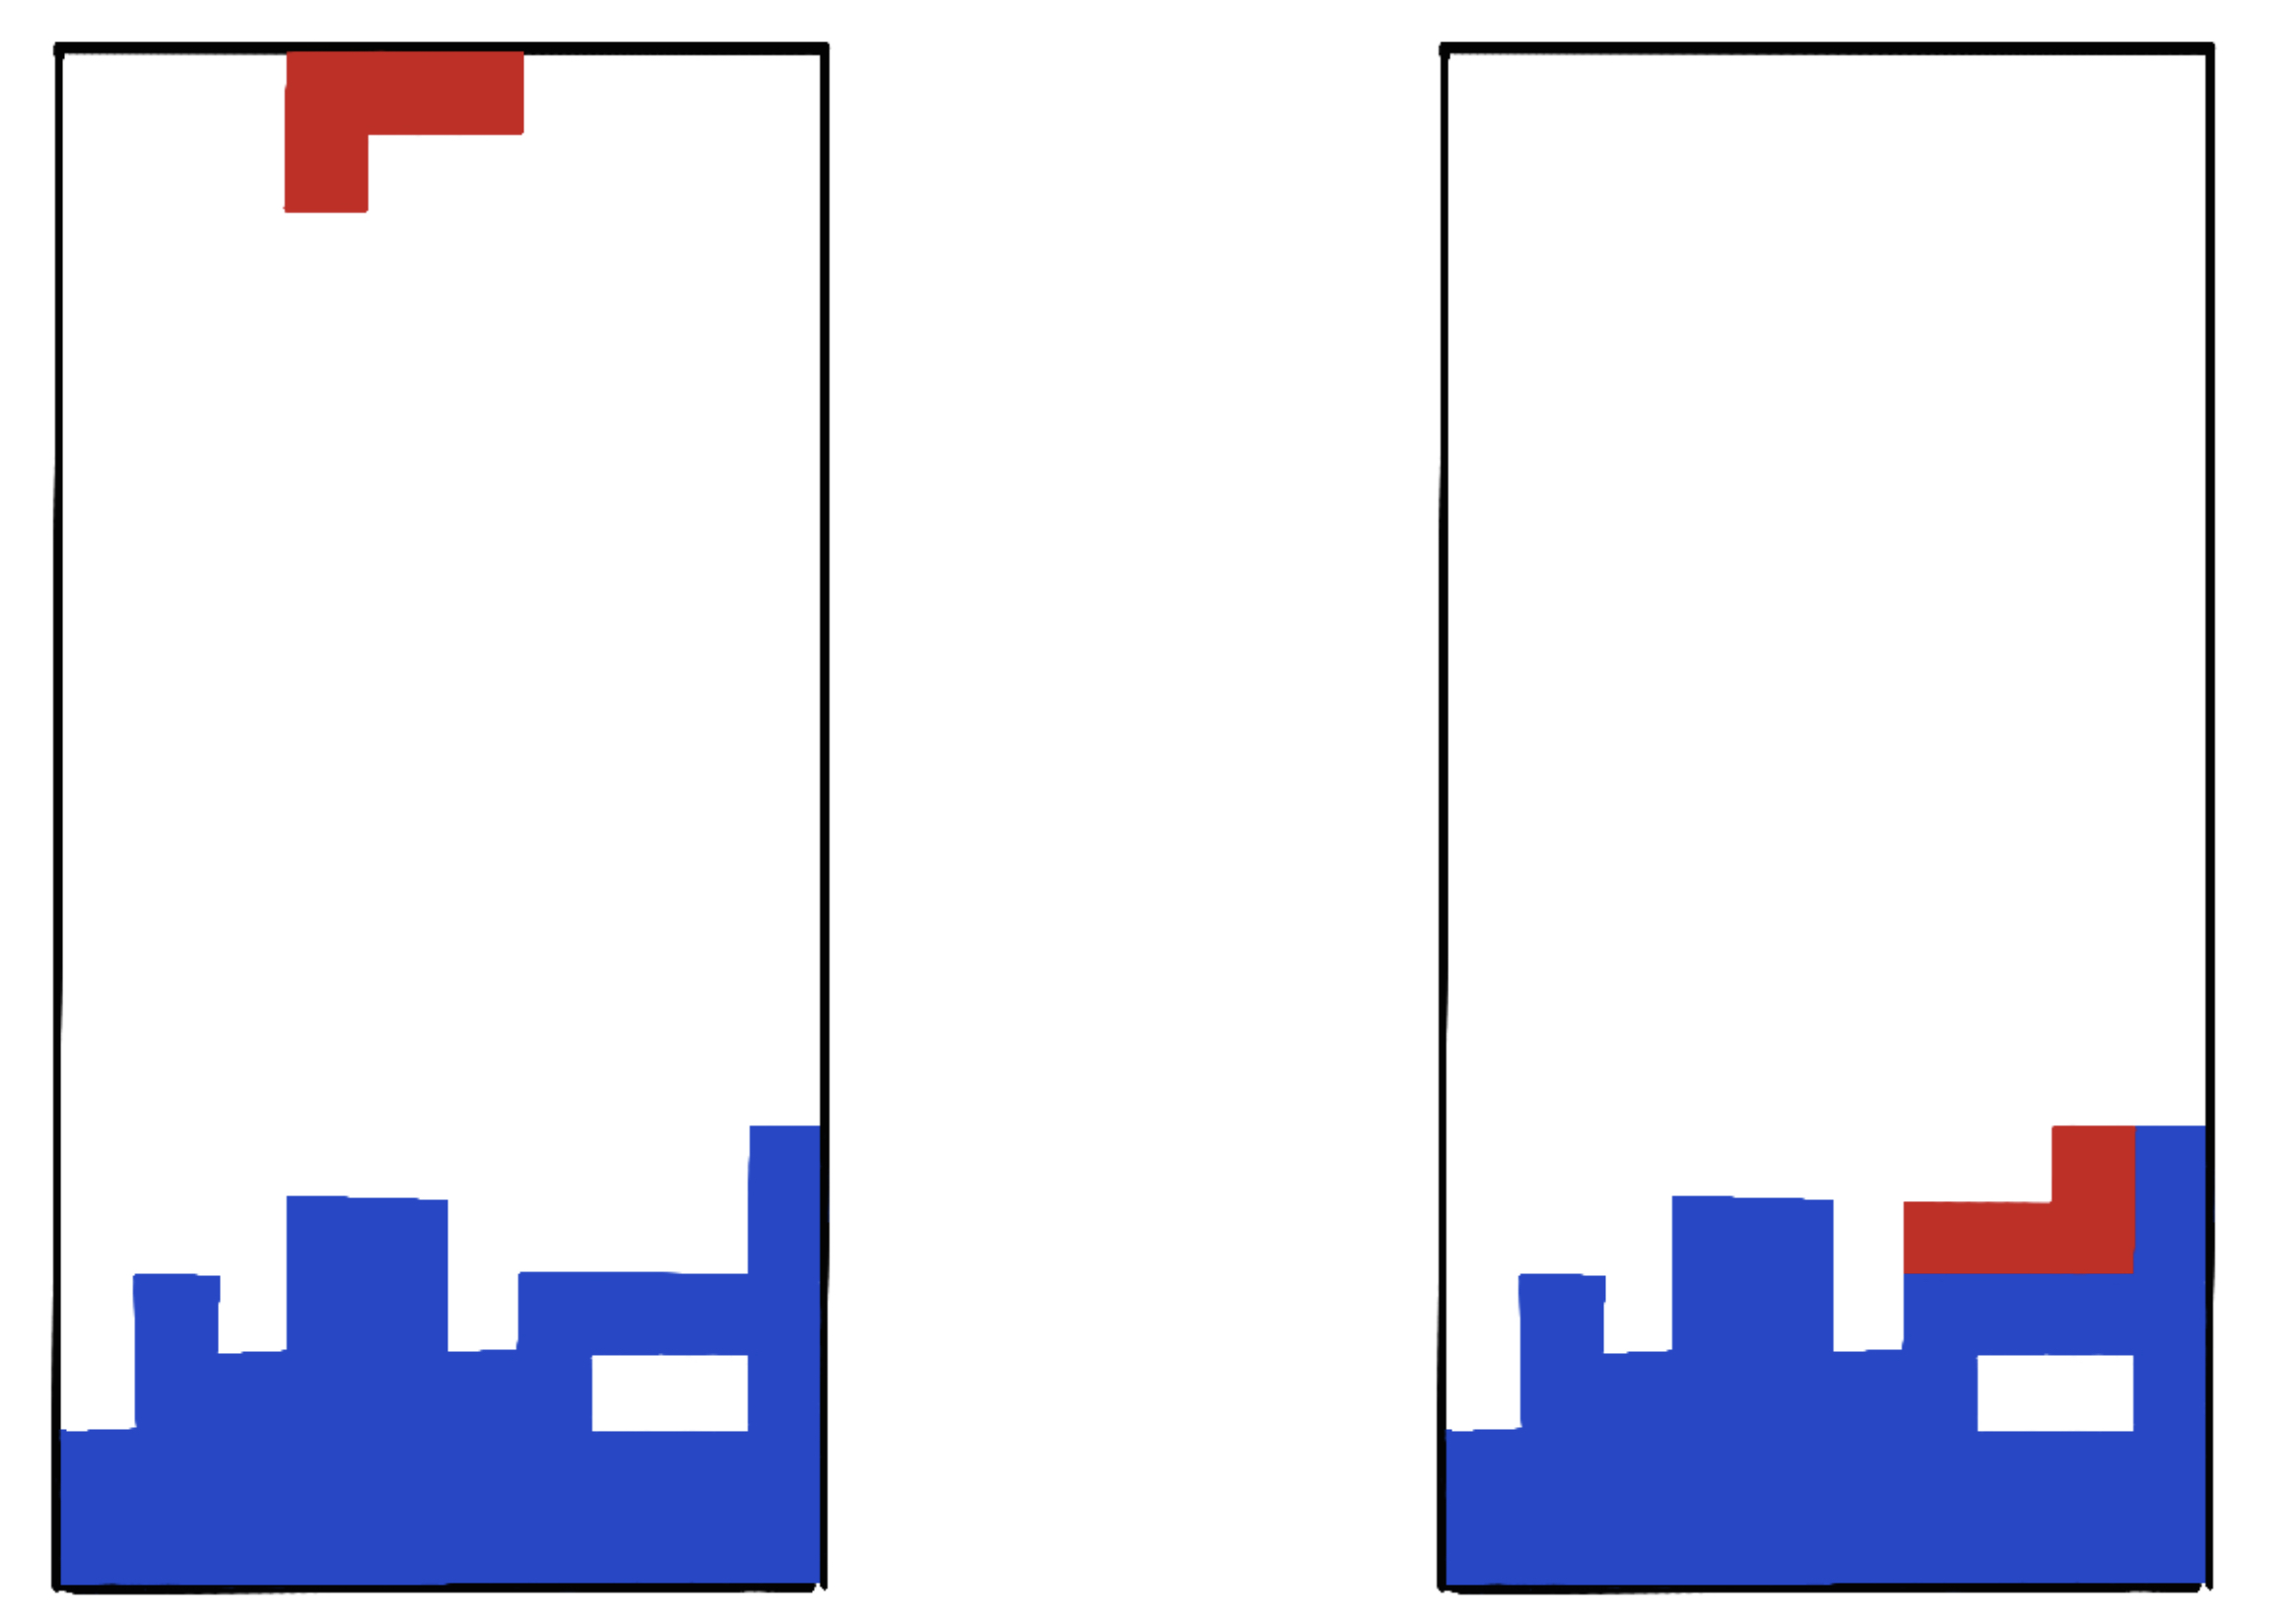
\includegraphics[width=0.9\linewidth]{figures/group_actions.jpeg}
  \caption{Grouped action example}
  \label{fig:grouped_action}
\end{figure}


\begin{figure*}[h]
  \centering
  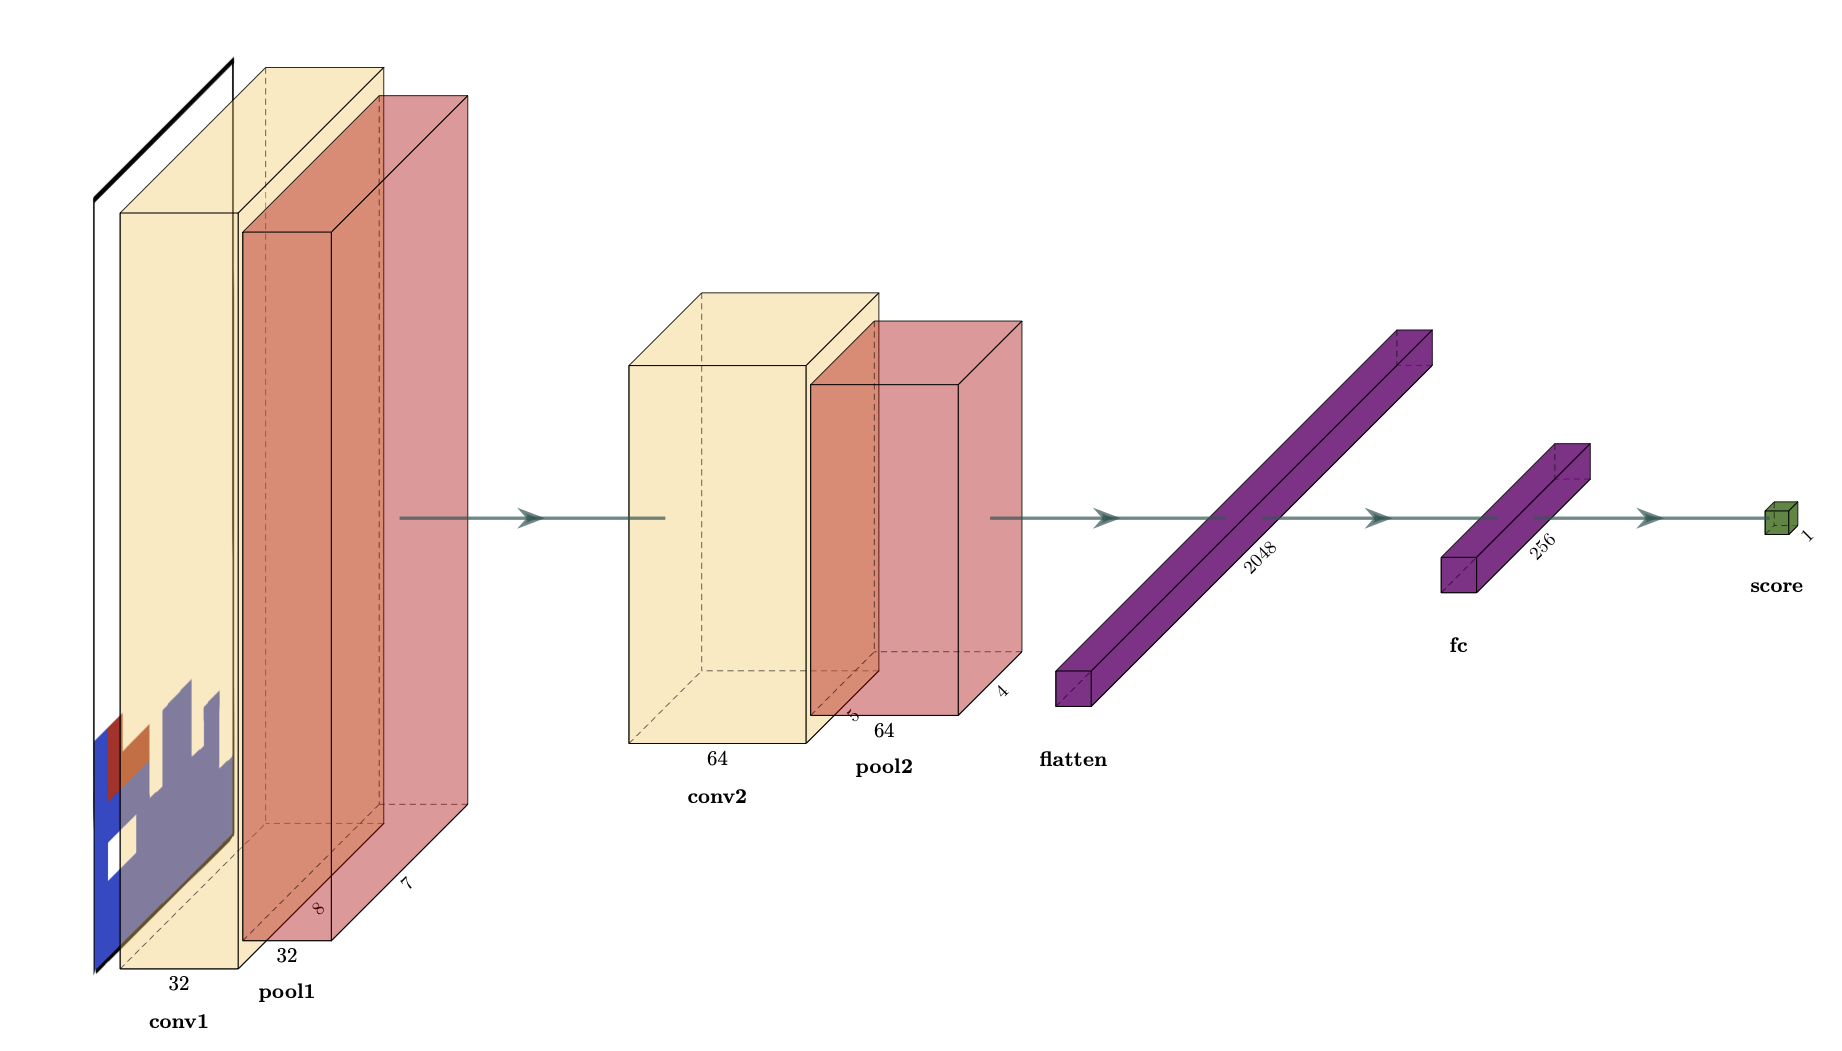
\includegraphics[width=0.85\linewidth]{figures/DQN.png}
  \caption{Deep Q-network architecture}
  \label{fig:DQN}
\end{figure*}

Now, we will conquer these two hindrances and develop a practical architecture for this problem. For the first one, inspired by Stevens and Pradhan's idea of \textit{grouped action}, we can leverage the successor function from the genetic algorithm and reduce the dimension of Q-table. More precisely, instead of defining action $a_i$ to be one of the $5$ single moves, we will use a \textit{grouped action} to represents a sequence of moves until the current Tetromino is landing. \footnote{In other words, each \textit{grouped action} refers to a final placement for a specific Tetromino.} For example, if we got an L-shape Tetromino as shown in Figure \ref{fig:grouped_action}, one potential \textit{grouped action} will be $\{left\times 4, \,\,clockwise\,\,rotation \times 2,\,\,down\times 12\}$, which is essentially the successor function from the genetic algorithm.


With the new definition of \textit{grouped action}, we can reconstruct our Q-table and rewrite our updating formula. Notice that because after each grouped action, it's guaranteed to be a stable state (i.e., there is no floating Tetromino), we can simplify the two-dimensional Q-table into one-dimensional:
\begin{table}[h!]
  \centering
  \normalsize{
    \begin{tabular}{ |c|c|c|c|c|c| } 
      \hline
      $s_{0}$ & $s_{1}$ & $\cdots$ & $s_{m-1}$ & $s_{m}$  \\ 
      \hline
      $0.91$ & $0.65$ &$\cdots $ &$0.45$ &$0.19$  \\ 
       \hline
      \end{tabular}}
  \caption{New Q-table with random initialization}
  \label{tab:qtbale}
\end{table}

with the modified updating formula:
\[
    % Q^{new}(s_{t},a_{t}) \leftarrow \underbrace{Q(s_{t},a_{t})}_{\textit{old value}} + \underbrace{\alpha}_{\textit{learning rate}} \cdot  \overbrace{\bigg( \underbrace{\underbrace{r_{t}}_{\textit{reward}} + \underbrace{\gamma}_{\textit{discount factor}} \cdot \underbrace{\max_{a}Q(s_{t+1}, a)}_{\textit{estimate of optimal future value}}}_{\textit{new value (temporal difference target)}} - \underbrace{Q(s_{t},a_{t})}_{\textit{old value}} \bigg) }^{\textit{temporal difference}}
    Q(s_{t}) \leftarrow (1-\alpha) Q(s_{t}) + \alpha   \left ( r_{t} + \gamma  \max_{s_{i} \in successor(s_{t})}Q(s_{i})\right ) 
\]

With the reconstructed Q-table and modified updating formula, now for each state, the agent will choose the successor with the highest Q-value instead of a specific action. This successfully solves the sparse reward problem because now, after each grouped action, we will always get a non-zero reward according to \ref{tab:reward}. However, this setup inherits the drawback of requiring enormous storage space and training time because the number of states remains $10^{60}$. 

To overcome the second hindrance, we need to understand why we have so many states in our Q-table. The problem lies in the fact that we have $20\times 10$ cells in the game board, and the number of possible states is exponential in the number of cells. This situation reminds us of how we encode images during image classification, and naturally, we will consider using Convolutional Neural Networks (CNN) to encoding our state (i.e., a $20\times 10$ bitmap).  This idea is first introduced by Google DeepMind in the paper Playing Atari with Deep Reinforcement Learning \cite{Mnih_2013}, and we will adapt this idea to Tetris to come up with the architecture as shown in Figure \ref{fig:DQN}.

Notice that this Deep Q-network (DQN) will take a $20\times 10$ bitmap as input and output a non-negative real number as the score for that bitmap. This behavior is essentially the same as what we did in Q-learning except that the DNQ will generate the score on the fly while Q-learning will merely look up the score. At its core, the DQN is trying to approximate the Q-table using a reasonable amount of time and space. 

Compared with other CNN architecture, our DQN is relatively small and straightforward, mainly because of the tiny input size. Here is a summary for each layer in Figure \ref{fig:DQN}:
\begin{itemize}
  \item 
  {\bf conv1}: a convolutional layer with filter size $3\times 3$, output channel size $32$, and leaky ReLU activation function.
  \item 
  {\bf pool1}: a max-pooling layer with filter size $2\times 2$.
  \item 
  {\bf conv2}: an identical layer as {\bf conv1} except that the output channel size to be $64$.
  \item 
  {\bf pool2}: an identical layer as {\bf pool2}.  
  \item 
  {\bf flatten:} this is simply a flattened version of the {\bf pool2} feature map.
  \item 
  {\bf fc}: this is a fully connected layer of size $256$ with ReLU activation function.
  \item 
  {\bf score}: this is a fully connected layer of size $1$ with ReLU activation function.
\end{itemize}

On top of that, here is the pseudo-code to train our DQN:

\begin{figure}[h!]
	\centering
	\begin{minipage}{.95\linewidth}
    \removelatexerror% Nullify \@latex@error
		\begin{algorithm}[H]
			\DontPrintSemicolon
			\SetKwFunction{FMain}{train}
			\SetKwProg{Fn}{Function}{:}{}
			\Fn{\FMain{$cur$, $DQN$}}{
      \textbf{Input: }$cur$ is current game state and $DQN$ is the network, which supports two operations $predict$ and $fit$\;
      \textbf{Input: }$nex$ is the next game state\;
      $states \gets successor(cur)$\;
      $maxQ \gets 0, reward \gets 0, maxState \gets \textbf{None} $\;
      \For{$state$ \textbf{in} $states$}{
        $score \gets DQN.predict(state)$\;
        \If{$score > maxQ$} {
          $maxQ \gets score$\;
          $reward \gets reward(state)$\;
          $maxState \gets state $\;
        }
      }
      $Q' \gets (1-\alpha) \cdot maxQ + \alpha  \cdot  \left ( reward + \gamma\cdot   maxQ\right )$\;
      $DQN.fit(maxState, Q')$\;
      \Return maxState\;
			}
		\end{algorithm}
	\end{minipage}
  \caption{Pseudo-code for Training}
\end{figure}

In summary, DQN architecture successfully solves the problems of sparse reward and enormous states, which gives us an efficient and effective estimation for the original Q-learning in Table \ref{tab:qtable}. Moreover, with CNN's powerful encoding capability, we don't need to choose the features manually, and the architecture will automatically find the optimal features during backpropagation. As a result, we can say that DQN architecture has the potential to outperform the genetic algorithm.

% {\bf Complete this section for D2.}

% The {\it Methodology } section ($\sim$2 pages) describes the algorithms that you chose to implement.  Describe in details how each algorithm works.  Include their mathematical formulations, if necessary.  Include pseudo-code, if necessary.  If you had to extend an existing algorithm in order for it to work with the problem, describe in details what is different/new.  Provide a rationale for why you selected these particular algorithms and how they are appropriate for the problem.  You should provide enough details so that someone can reproduce the steps and replicate your results.  

% If you are tackling a machine learning problem, you may be using an existing data set or creating a new data set.  In this case, you should describe the data-set that you are analyzing as well as any data filtering and merging procedures that you used to prepare/create your data-set.  Your description should. include the size of the data-set(s) (i.e., number of examples), whether the class labels are balanced/imbalanced, the meaning of the features, and other unique characteristics of the data-sets.   Explain why the data-sets are appropriate for your problem and what are their limitations.  Include the URL of the websites from which you downloaded the data-set(s).

% You should also describe any pre-processing steps you took to prepare or create the final data-set that you used to train and test the algorithms.  Examples of pre-processing steps include procedures for joining multiple data-sets, filtering out certain examples, scaling features, etc.  Provide the rationale for why you are using these data preparation procedures, with enough details so that someone can reproduce the steps and replicate your results.   For example, if you chose to re-scale certain features, explain how the re-scaling was done and why.   


%%%%%%%%%. Example of subfigure and 2-column figure layout %%%%%%%%%

\begin{figure*}[t!]
\centering
\subfigure[image A]{
\fbox{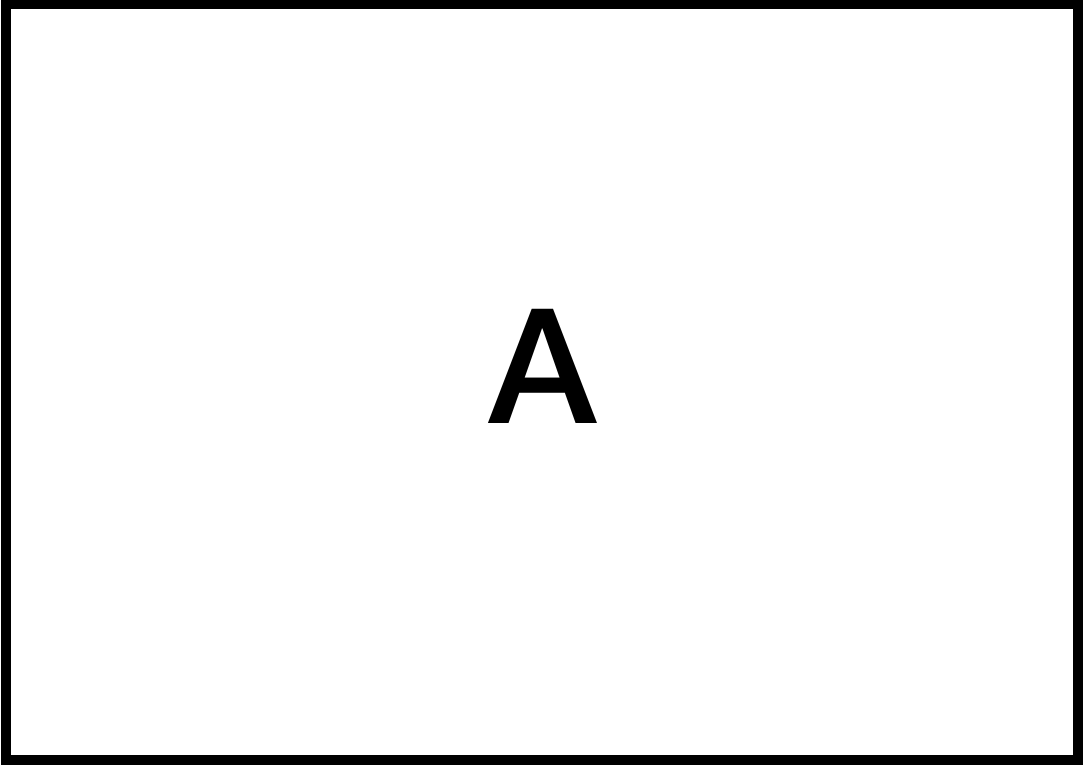
\includegraphics[height=2.6cm]{figures/A}}
\label{fig:a}
}\hfill
\subfigure[image B]{
\fbox{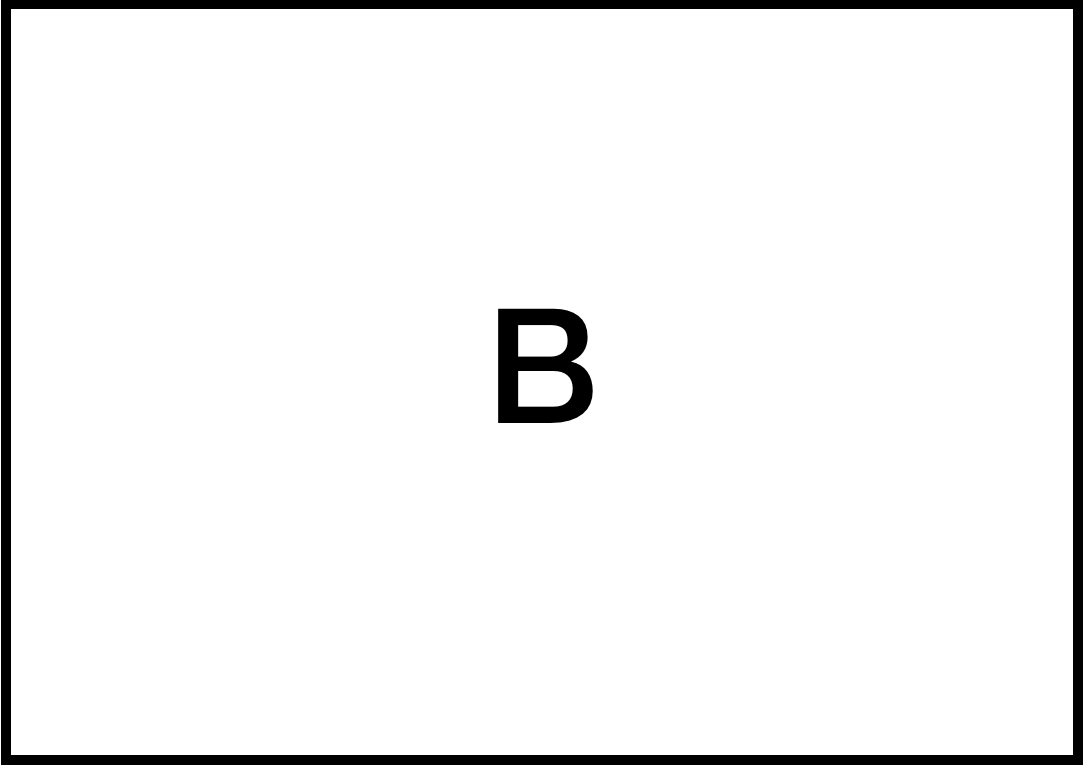
\includegraphics[height=2.6cm]{figures/B}}
\label{fig:b}
}\hfill
\subfigure[image C]{
\fbox{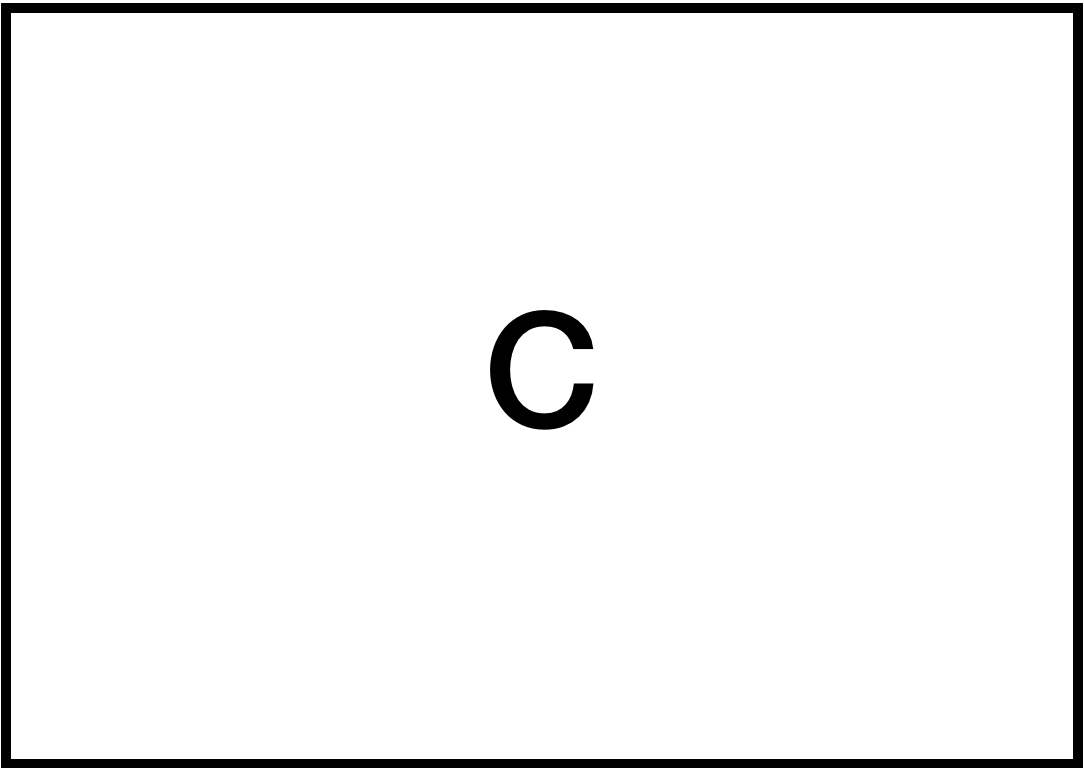
\includegraphics[height=2.6cm]{figures/C}}
\label{fig:c}
}\hfill
\subfigure[image D]{
\fbox{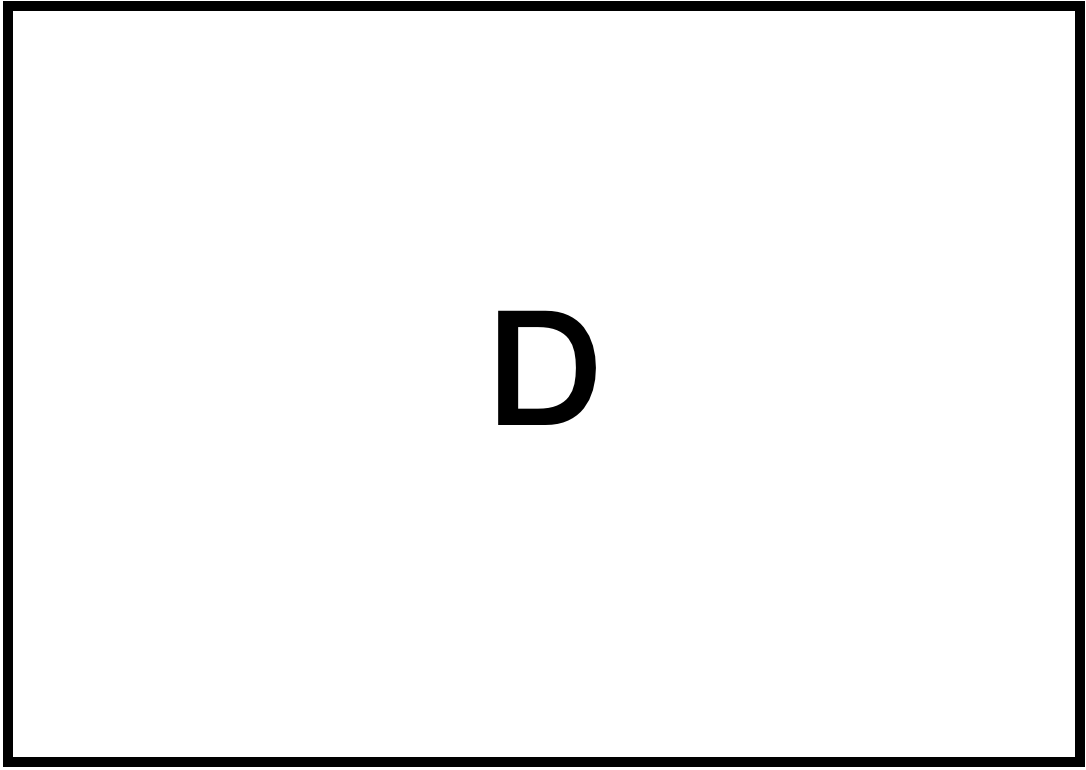
\includegraphics[height=2.6cm]{figures/D}}
\label{fig:d}
}\hfill
\caption{Another example of figure layout}
\label{fig:figures_across}
\end{figure*}

%%%%%%%%%. Results %%%%%%%%%

\section{Results}
\subsection{Environmental Setup}
\subsection{Evaluation Metrics}
Describe the measures that you used to evaluate the algorithms.  Be as precise as possible by including their mathematical formulations.  Provide a rationale for why these performance metrics are appropriate for your problem.
\subsection{Experimental Designs}
Describe other details about your experimental design.  If you are tackling a machine learning problem, include details such as how you created the training, validation and test set, how you selected the model's hyper-parameters, etc.    
\begin{itemize}
  \item \textbf{Handcrafted Agent} 
  \item \textbf{Local Search Agent} 
  \item \textbf{Reinforcement Learning Agent} 
\end{itemize}
% {\bf Complete this section for D2 and D3.}

% The {\it Results} section ($\sim$2 pages) describes how you evaluated the algorithms and reports the findings.  

% {\bf Complete the following two paragraphs for D2.}



{\bf Complete the following two paragraphs for D3.}

Describe the findings from your evaluation.  Describe both (a) how well your techniques worked, and (b) what you learned about the problem through these techniques.  

Prepare figures (e.g., Figure \ref{fig:results2}) and tables (e.g., Table \ref{tab:results1}) to describe your results clearly.  Make sure to label your figures and tables and explain them in the text.  If you are comparing the performance of algorithms, include statistical tests to assess whether the differences are statistically significant.  If possible, describe how your techniques compare to prior work.  

\begin{table}[h!]
    \centering
    \normalsize{
    \begin{tabular}{ l c }
    \hline
         Techniques & F-1 Score\\
         \hline
          Baseline & 0.80 \\
          Another Baseline & 0.76\\
          My Awesome Algorithm & {\bf 0.95}\\
         \hline
    \end{tabular}}
    \caption{example of a table summarizing the results}
    \label{tab:results1}
\end{table} 

\begin{figure}[htbp!]
  \centering
  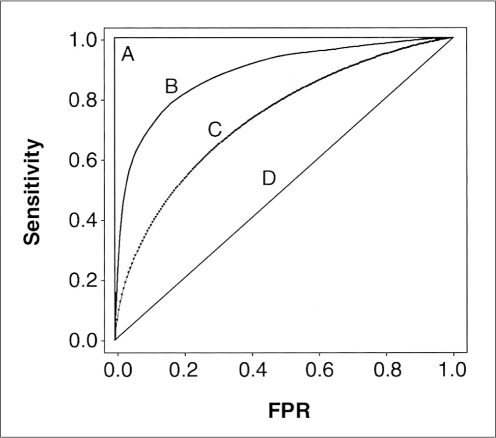
\includegraphics[width=0.9\linewidth]{figures/roc.png}
  \caption{ROC curve of my awesome algorithms}
  \label{fig:results2}
\end{figure}


%%%%%%%%%. Discussion %%%%%%%%%

\section{Discussion}

{\bf Complete this section for D4.}

The {\it Discussion} section ($\sim$1 pages) describes (a) the implications of your results, and (b) the impact and the limitations of your approach.  

For the results, describe how a reader should interpret them.  Try to form concise take-away messages for the reader.  For your approach, describe the extent to which your approach helps to solve the problem.  Describe any limitations of your approach.  If possible, compare your results and your approach to that of prior work. 

%%%%%%%%%. Conclusion %%%%%%%%%

\section{Conclusion}

{\bf Complete this section for D4.}

The {\it Conclusion} section ($\sim$0.5 pages) provides a brief summary of the entire paper.  In this section, describe 
\begin{itemize}
    \item the motivation, the problem, and your results, and
    \item 3-4 promising future directions.
\end{itemize}

%%%%%%%%% Bibliography %%%%%%%%%
\newpage
\bibliographystyle{aaai}
\bibliography{report}

\end{document}
